\chapter{Architecture}

\section{Introduction}

\section{Prototype}
For demonstrating the architecture of this project we implement an architecture
prototype which shows basic functionality of producing a message from a client A
to persisting the message in a  topic specific log at the broker and in turn consuming it from another
client B. It fully implements the produce and fetch request with their
appropriate responses of the Kafka protocol for communication over network.
Therefore the producer and consumer clients are compatible with original Apache
Kafka broker.

The functionality of the architecture prototype can be split in two cases.
Case one covers producing a message and persisting in the brokers log:
\begin{figure}[H]
    \centering
    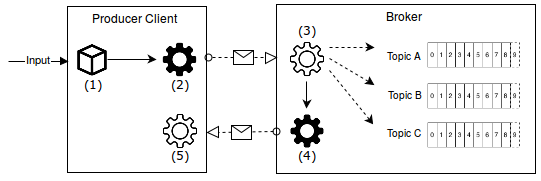
\includegraphics[width=0.8\textwidth]{images/concept_producer.png}
    \caption{Concept of Architecture Prototype Part I}
    \label{fig:conept-producer}
\end{figure}

\begin{table}[h]
\begin{tabular}{ll}
1  & Packing input message in data structure                                                          \\
2  & Serializing of data structure to byte string. The algorithm implements the Kafka protocol.       \\
3 & Transmitting byte string via TCP socket over network                                             \\
4  & Receiving and parsing byte string back to data structure                                         \\
5   & Write Message into topic specific log. The resulting file has same structure than the Kafka Log has.
\end{tabular}
\end{table}

Case two covers the part of consuming from a specific topic. Because Kafka works with 
pull-based consumption, the consumer fetch its messages with a constantly requesting it. 

\begin{figure}[H]
    \centering
   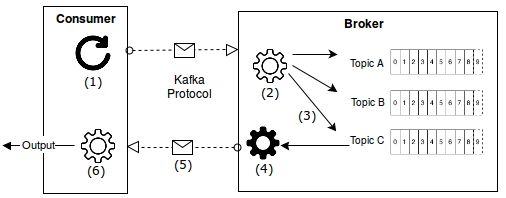
\includegraphics[width=0.7\textwidth]{images/concept_consumer.png}
    \caption{Concept of Architecture Prototype Part II}
    \label{fig:concept-consumer}
\end{figure}

\begin{table}[h]
\begin{tabular}{ll}
1  & Continuously send fetch request to broker implementing Kafka protocol \\
2  & Parse fetch request to data structure                                 \\
3  & Read messages from log of specified topic                             \\
4  & Serialize messages as response into byte string.                      \\
5  & Transmitting byte string back to consumer                             \\
6  & Parse response from broker to get messages                           
\end{tabular}
\end{table}

\section{Components}
Basically, the architecture consists of two main components namely the broker and
the client, whereas the client can act as producer or consumer. The broker is a
server which only reacts to requests that are sent from clients. Every request
contains an API Key which the broker uses to determine which action it has to
do (e.g. persist produced message or consume message). For each request the
broker sends back a corresponding response to the client which either includes
the fetched data or an error code. The broker never communicate with a
client without a request.

\begin{figure}[H]
    \centering
     \begin{sequencediagram}
        %\newthread{broker}{Broker}
         \newinst[3]{client}{Client}
         \newinst[3]{broker}{Broker}
        \begin{messcall}
            {client}{(1) Send Request}{broker}{}
        \end{messcall}
        \begin{messcall}
            {broker}{(2) Do Action}{broker}{}
        \end{messcall}
        \begin{messcall}
            {broker}{(3) Send Response}{client}{} 
        \end{messcall}
     \end{sequencediagram}
     \caption{Basic communication between client (producer or consumer) and
     broker}
\end{figure}

Both, the client and broker component need to use the same protocol for
communication. Therefore a third component which fully implements the Apache Kafka
protocol \todo{ref} and provides the appropriate functions and types to the
broker and clients comes into game. Further this component separates the client
from the broker wheres the clients also can be used to work with other broker
implementations especially original Apache Kafka. 

A good broker system should have as many client implementation as possible to
support lot of applications in different languages. As basic clients a simple
console-producer and console-consumer is provided but to support the development
of other clients a fourth component which act as common client api ist
introduced. It provides common functionality to simplify the use of the protocol
implementation. 

\begin{figure}[H]
    \centering
    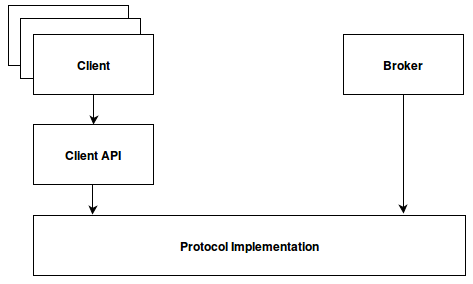
\includegraphics[width=0.55\textwidth]{images/architecture-components.png}
    \caption{Components of the architecture}
    \label{fig:architecture-components.png}
\end{figure}

\section{Protocol}
\label{sec-protocol}
For communicating over network we implement a binary protocol based on tcp. The
structure of the protocol is identical to the open sourced Apacke Kafka protocol
version 0.8.x. \todo{ref}The protocol offers six different apis which each of it is
defined with a request response message pair. The client initiates a socket connection and then
writes a sequence of request messages and reads back the corresponding response
message. 

\subsection{Primitive Types}
All messages are size delimited and are made up of the following primitive
types: 

\begin{table}[h]
\begin{tabular}{| p{3cm}| p{7cm} | l |}
\hline
\textbf{Type} & \textbf{Description} & \textbf{Variations} \\ \hline
Fixed Width Primitives     & Signed integers stored in big endian order.                                                                                                                                     & int8, int16, int32, int64 \\ \hline
Variable Length Primitives & Consist of a signed integer giving a length N followed by N bytes of content. A length of -1 indicates null. String uses an int16 for its size, and bytes uses an int32.        & bytes, string             \\ \hline
Arrays                     & Repeated structures. Always be encoded as an int32 size containing the length N followed by N,repetitions of the structure which can itself be made up of other,primitive types &                           \\ \hline
\end{tabular}
\end{table}

\subsection{Common Message Format}
The message as unit of transported data has the following common structure of a
message set which is used for all api's which transport message data.
Furthermore this format happens to be used both for the on-disk storage on the
broker and the on-the-wire format.

\begin{figure}[H]
    \centering
    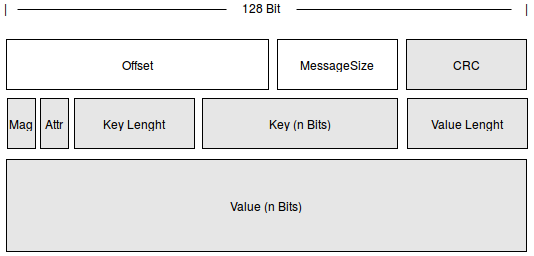
\includegraphics[width=0.7\textwidth]{images/protocol-messageSet.png}
    \caption{Message Set format as common data structure}
    \label{fig:protocol-request-header.png}
\end{figure}

\subsection{Common Request and Response Header}
Each request and response has its same header fields independent for which api they are used. 
The last part of the format (either request or response) is individual to the particular api which is used. 
\begin{figure}[H]
    \centering
    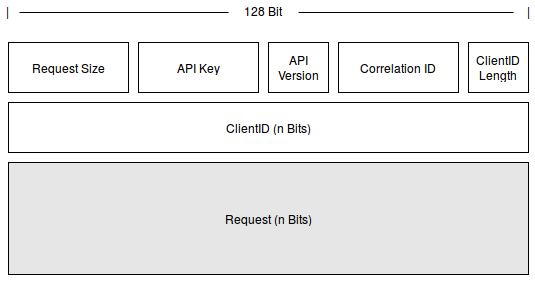
\includegraphics[width=0.7\textwidth]{images/protocol-request-header.png}
    \caption{Common Request Header}
    \label{fig:protocol-request-header.png}
\end{figure}

\begin{figure}[H]
    \centering
    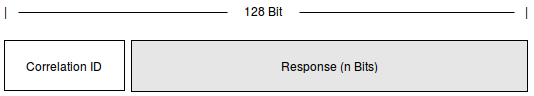
\includegraphics[width=0.7\textwidth]{images/protocol-response-header.png}
    \caption{Common Request Header}
    \label{fig:protocol-response-header.png}
\end{figure}

\subsection{Metadata API}
Describes the currently available brokers, their host and port information, and
gives information about which broker hosts which partitions.

\textbf{Not implemented yet}

\subsection{Produce API}
Send messages to the broker.

\textbf{Not implemented yet}

\subsection{Fetch API}
Fetchs / Consumes messages from the broker.
\subsection{Offset API}
Get information about the available offsets for a given topic partition

\textbf{Not implemented yet}

\subsection{Offset Commit API}
Commit a set of offsets for a consumer group

\textbf{Not implemented yet}

\subsection{Offset Commit API}
Fetch a set of offsets for a consumer group

\textbf{Not implemented yet}

\section{Packages, Modules and Dependencies}
\todo[inline]{how did we structure the executables ans libraries}

The application has three main parts namely the broker, protocol implementation
and the client api. 
%Each part is built in its own self-contained cabal package.

\begin{figure}[H]
    \centering
   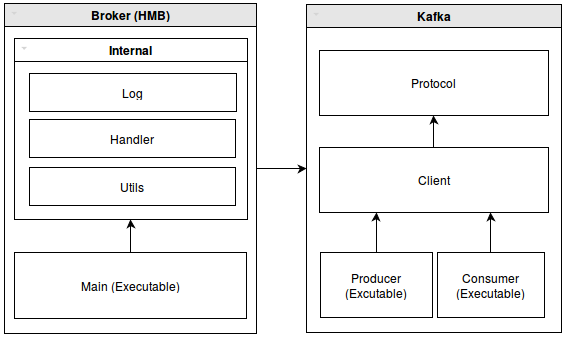
\includegraphics[width=0.7\textwidth]{images/logical-architecture.png}
    \caption{Package structure and dependencies}
    \label{fig:logical-architecture}
\end{figure}

\subsection{Protocol Implementation}

\subsubsection{Types}

The design of the Apache Kafka protocol allows to make a distinction between three kind of types:
\begin{enumerate}
  \item Related to request
  \item Related to response
  \item Related to data (for either request or response but can also be used for the \fnurl{Apache Kafka Log}{http://kafka.apache.org/documentation.html\#log} component since log files (on-disk) hold the same structure)
\end{enumerate}

As for request and response related types we had to introduce an own naming
convention. As a matter of fact, not every field of some kind of request or
response will be unique. For more than once, there is a field that will
represent a \textit{topicName} for example. Thus, naming the field \textit{
topicName} would have been the obvious solution but since the record syntax in
Haskell won't allow to use the same name for a field twice - even in different
data types - we defined unique prefixes for each request and response as being
listed in the following table:

\begin{table}[h]
\centering
\begin{tabular}{|l|l|l|}
\hline
\textbf{API}            & \textbf{Request (Rq)} & \textbf{Response (Rs)} \\ \hline
Metadata API (Md)       & MetadataRequest       & MetadataResponse       \\ \hline
Produce API (Pr)        & ProduceRequest        & ProduceResponse        \\ \hline
Fetch API (Ft)          & FetchRequest          & FetchResponse          \\ \hline
Offset API (Of)         & OffsetRequest         & OffsetResponse         \\ \hline
Offset Commit API (Ofc) & OffsetCommitRequest   & OffsetCommitResponse   \\ \hline
Offset Fetch API (Oft)  & OffsetFetchRequest    & OffsetFetchResponse    \\ \hline
\end{tabular}
\end{table}

As mentioned before, the representation of the protocol structure is
implemented using the Haskell \fnurl{type
system}{https://wiki.haskell.org/Type}, more concrete using data types created
for our need using the named fields - also known as \fnurl{record
syntax}{http://en.wikibooks.org/wiki/Haskell/More_on_datatypes}.

Given this, a further step of abstraction is introduced by creating types for the binary representation of a protocol field.
The actual type for the data fields in the protocol have to match an unsigned integer type of its length. This can easily be done using the \fnurl{Data.Word}{http://hackage.haskell.org/package/base-4.7.0.2/docs/Data-Word.html} library.
However, while repetitive writing \textit{WordX} (where is stands for 8-, 16-, 32-, or 64 bit) is rather intuitive, creating aliases using the \textit{type} keyword will result in better readable code, as well as structure of the implemented protocol.

\subsection{Encode / Decode}

\subsection{Client (API)}

\section{Error Handling}

\section{Testing}
hspec 

\section{Client Examples}
This example shows a very basic console client which either can act as producer
by sending a producer request or as a consumer by sending a fetch request. After
sending the client wait for a corresponding response from the broker.

Init stream socket an open connection to a given host address and port (broker must be running on same ip and port): 
\begin{lstlisting}
  sock <- socket AF_INET Stream defaultProtocol 
  setSocketOption sock ReuseAddr 1
  putStrLn "Give IP"
  ipInput <- getLine
  let ip = toHostAddress (read ipInput :: IPv4)
  putStrLn "Give Port"
  port <- getLine
  connect sock (SockAddrInet port ip)
\end{lstlisting}
\todo{port convertierung}

If connection succeeded give client id and topic name: 
\begin{lstlisting}
  putStrLn "Give Client Id"
  clientId <- getLine
  putStrLn "Give Topic Name"
  topicName <- getLine
\end{lstlisting}

Producer: Sends given message to the broker. Client API function packPrRqMessage
packs the input into a protocol conform produce request, whereas the function
sendRequest encodes the request an send it over given socket connection.
Afterwards a response from broker is expected. If there is a response the client
can decode it with the API function decodePrResponse. 
\begin{lstlisting}
  forever $  do 
    putStrLn "Nachricht eingeben"
    inputMessage <- getLine
    sendRequest sock $ packPrRqMessage (clientId, topicName, 0, inputMessage)

    input <- recv sock 4096
    let response = decodePrResponse input
    print response 
\end{lstlisting}

Consumer: Send a fetch request with given offset to the broker. Analog to the producer request 
the api function packFtRqMessage packs the input into a protocol conform fetch request and sendRequest passes it via socket to the broker. 
\todo{code not final yet}


